\documentclass{clv3}

\usepackage{hyperref}
\usepackage{xcolor}
\definecolor{darkblue}{rgb}{0, 0, 0.5}
\hypersetup{colorlinks=true,citecolor=darkblue, linkcolor=darkblue, urlcolor=darkblue}

\bibliographystyle{compling}


% test compatibility with algorithmic.sty
\usepackage{algorithmic}
\usepackage{ctex}
\usepackage{amsmath}
\usepackage{amssymb}
\usepackage{caption}
\usepackage{graphicx}

\issue{1}{1}{19}

%Document Head
\dochead{自然语言处理19-20秋季课程作业} % 修改此处
%
\runningtitle{自然语言处理19-20秋季课程作业} % 修改此处
%
\runningauthor{曾四为} % 修改此处

\begin{document}

\title{多轮对话综述:过去、现在与应用} % 修改此处

\author{曾四为} % 修改此处
\affil{中国科学院大学} % 修改此处


\maketitle

\begin{abstract} % 修改此处
对话系统旨在使机器能够通过自然语言与人类沟通,从而充当虚拟助手和智能客服等角色来为人们提供生活中的便利性。在自然语言处理领域,对话系统是一个广受关注的研究方向。随着深度学习的发展,对话系统能够利用大规模数据深层次地学习语句的特征表示和回复策略,展现出越来越大的应用潜力。本文沿着研究的发展历史来全面总结对话系统各个阶段的模型,并对当前工业级对话系统应用模型进行简单地描述。
\end{abstract}

\section{引言} % 修改此处
$\qquad$自从1950年图灵提出正式的人工智能测验\cite{turing1950i}后,创建一个能够和人自然、流畅交流的对话系统就成为自然语言处理领域的一个重要目标,同样也是一项具有挑战性的工作。

对于对话系统,根据不同的分类标准,有不同的划分方式。
根据其应用领域,可以分为问答对话系统、闲聊对话系统和任务对话系统\cite{chen2017a};
根据其涉及的领域,可以分为开放领域对话系统和垂直领域对话系统;根据其是否使用历史对话信息,可以分为单轮对话系统和多轮对话系统\cite{shang2015neural, mou2016sequence};
根据研究的发展历史和系统构建方式,可以分为第一代基于符号规则和模版的对话系统、第二代基于管道的对话系统和第三代大数据驱动的对话系统。

\subsection{问题描述}
$\qquad$对话系统的形式化描述为:每一次用户与计算机的交互会话中,都是用户以一句自然语言所构成的话语作为输入(也可称为查询),计算机返回一句用户可以理解的回答。多轮对话系统会利用会话中的历史对话信息,而单轮对话系统只根据当前用户输入给出回答。

记用户的输入为$q$,系统的回复为$r$,对话历史信息为$c$,对话系统的回复获取过程为$f$:
\vspace{-10pt}
\begin{itemize}
	\setlength{\itemsep}{0pt}
	\item 对于单轮对话系统有:$r=f(q)$
	\item 对于多轮对话系统有:$r=f(q, c)$
\end{itemize}

对于不同的对话系统,主要有三种回复获取方式:
通过对话状态根据模版进行回复的填充和生成;
将查询与语料库中的查询-回复对进行匹配,通过检索返回匹配度最高的结果;
通过文本生成的方法,根据查询生成出对应回答。



\subsection{本文框架}
$\qquad$本文旨在(1)按照对话系统的发展历史,对对话系统进行全面的的回顾分析;(2)对工业界对话系统进行简要介绍。本文在第2节介绍基于符号规则和模版的对话系统;
第3节介绍传统统计模型以及当前流行的深度模型在基于管道的对话系统中的应用;第4节梳理大数据驱动下对话系统的两种端对端构建方法;第5节介绍当前工业界对话系统的设计架构;第6节是总结。

\section{第一代:基于符号规则和模版的对话系统}
$\qquad$最早期对于对话系统的研究\cite{weizenbaum1966eliza, wilensky1988the}集中在基于符号规则和模版的对话系统方向。对话系统通过人工规则对用户语句进行匹配,之后根据模版作出回应。

这类系统\cite{epstein2008parsing, marietto2013artificial}依赖于专家人工语法规则,具有规则解释性好、系统易编写易维护、漏洞易修正的优点。但是其缺点主要有三点:一是依赖于专家的人工规则设计,专家水平和规则质量高低严重影响系统质量,二是难以跨领域迁移,只能针对狭窄的垂直领域,三是构架成本高,需要消耗大量人力资源和时间成本。



\section{第二代:基于管道的对话系统} % 修改此处
\begin{figure}[h] %figure环境,h默认参数是可以浮动,不是固定在当前位置。如果要不浮动,你就可以使用大写float宏包的H参数,固定图片在当前位置,禁止浮动。
    \centering %使图片居中显示
    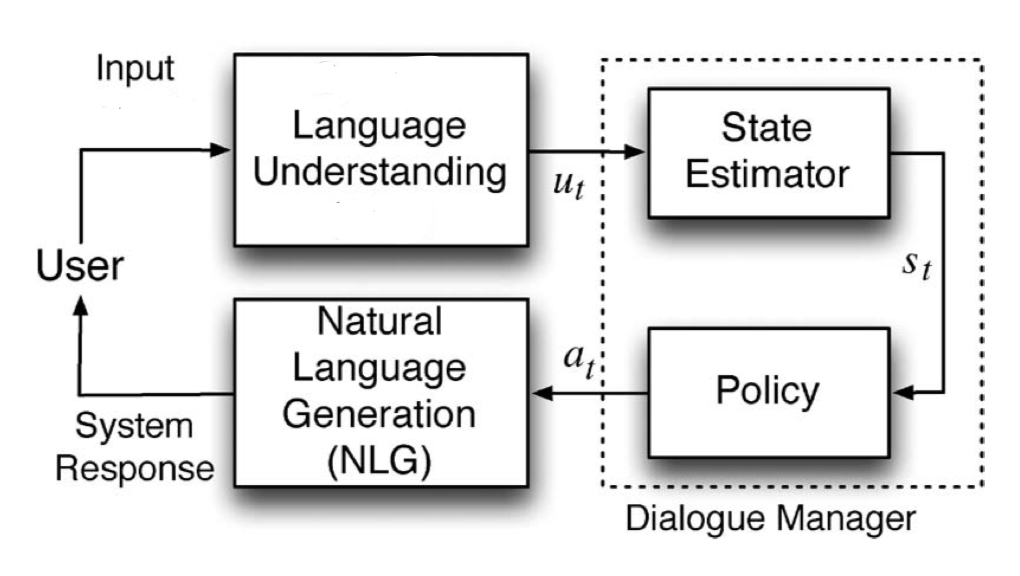
\includegraphics[width=1\textwidth]{pipeline_model} %中括号中的参数是设置图片充满文档的大小,你也可以使用小数来缩小图片的尺寸。
    \caption{基于管道的对话系统架构图} %caption是用来给图片加上图题的
    \label{pipeline_model} %这是添加标签,方便在文章中引用图片。
\end{figure}%figure环境
$\qquad$基于管道的对话系统的典型结构如图\ref{pipeline_model}所示,包含自然语言理解模块、对话状态追踪模块、对话规则学习模块和自然语言生成模块四个基本组件\cite{rudnicky1999creating, zue2000juplter, zue2000conversational}。
自然语言理解模块将用户的语句转换成预定义的意图和语义槽。对话状态追踪模块根据当前语句和对话历史,输出当前的对话状态;对话规则学习模块会基于当前的状态,执行相应的系统行为;自然语言生成模块根据系统行为的返回结果,生成用户能够理解的语句。
对话状态追踪模块和策略学习模块也被合称为对话管理模块。

基于统计的管道对话系统因为将人工规则和统计数据相结合,也被称为“数据驱动的对话系统”或“基于浅层学习的对话系统“。
得益于统计模型的应用,对话系统极大的减少了编写大量人工规则所带来的成本,并可以通过新的数据提升系统的表现。
但是统计对话系统一方面不容易理解和修补漏洞,另一方面学习能力不强,不能生成出符合人们预期的回复。

随着深度学习应用到NLP的各个领域,统计对话系统中各个模块的统计学习模型也逐渐被深度学习替代,但四个组件的整体结构没有变化。
\cite{zhao2016towards}提出第一个使用端到端强化学习方法来训练对话管理模块的模型。
\cite{wen2017a}和\cite{bordes2017learning}构建端到端的任务对话系统。


\subsection{自然语言理解模块}
自然语言理解模块需要根据用户问句提取出句子层次和词汇级别两个层次的信息,句子层次的信息包含句子的主题以及用户目的,而词汇级别的信息包含命名实体、动作的施事方和受事方等等。

\subsubsection{意图检测}
意图检测是指根据用户的语句,将其划分到预定义的某一个意图类中,从而起到检测用户意图的目的。
研究人员使用的传统统计模型有朴素贝叶斯分类器、逻辑斯特回归分类起、决策树模型和支持向量机等。

深度学习的技巧已经成功的应用到意图检测任务中。
研究人员使用DBN\cite{sarikaya2011deep}、DCN\cite{tur2012towards}、kernel DCN\cite{deng2012use}、RNN\cite{ravuri2015recurrent}和CNN\cite{xu2013convolutional}等深度模型来完成对用户语句的潜在意图识别。

\subsubsection{槽填充}
槽填充是指将用户语句中的每个词标注上一个语义标签,通常被认为是序列标注问题。
对于一个输入和句子,经过槽填充过程后会得到一个等长的标签序列。

研究人员使用条件随机场\cite{wang2006discriminative, raymond2007generative}、DBN\cite{deoras2013deep}和RNN\cite{yao2013recurrent, mesnil2013investigation}等模型来完成槽填充任务。
\cite{simonnet2015exploring}引入编码解码器结构和注意力机制来编码语句。
\cite{liu2016attention}将意图检测和槽填充任务结合,通过序列到序列模型或基于注意力机制的RNN所得到的隐状态同时完成两项任务。
\cite{zhai2017neural}结合指针网络,使得模型能够实现词组级别的槽位识别。

在经典数据集上\cite{hemphill1990the, dahl1994expanding},许多深度模型\cite{liu2016attention, zhai2017neural}都达到了95\%的准确性。为了进一步评估模型的能力,在槽填充领域还需要更多样化、更大规模的数据集。

\subsection{对话状态跟踪模块}
$\qquad$对话状态跟踪是确保对话系统健壮性的核心组件,通过被称为语义框架的状态结构来维护用户的当前会话状态。
具体来说,会话状态是通过对话历史、用户意图和槽值对构成的语义框架来描述。
对话跟踪模块根据每一轮次新的输入,对当前用户的状态进行更新,管理每个回合的输入和对话历史,输出当前对话状态。

基于规则的的模块构建方法已经在大多数商业实现中得到了广泛的应用,通常采用手工规则来选择最有可能的输出结果\cite{goddeau1996a}。
然而,基于规则的模块容易出现频繁的错误,因为实际对话往往不会按照人为设计的流程发展\cite{williams2013multi}。

基于统计的状态跟踪模块会根据当前会话状态对真实的对话状态计算一个概率分布\cite{williams2013the},用来处理充满噪音或模糊语义的情况。
多种统计方法都被使用,包括人工规则\cite{wang2013a}、条件随机场\cite{ren2013dialog, lee2013structured, kim2014sequential}、最大熵模型\cite{williams2013multi}和基于随机游走\cite{williams2014web}的排序模型。

\cite{henderson2013deep}利用DNN在时间窗口内对多轮状态提取的特征。
\cite{mrkšić2015multi}用RNN进行多领域的对话状态追踪,并证明利用多个领域的数据有助于模型表现提升。
\cite{mrksic2017neural}通过将所有槽位和当前状态经过编码后的语义表示逐一进行相关性二分类。


\subsection{策略学习模块}
$\qquad$策略学习根据状态跟踪器的状态表示生成下一个可用的系统动作(action)。
在在线购物场景中,如果对话状态是“推荐”,那么触发“推荐”操作,系统将从产品数据库中检索产品。

无论是人工规则、监督学习还是强化学习都可以用来优化策略学习\cite{cuayáhuitl2015strategic}。
然而,基于规则的模块面对巨大的状态空间容易出现错误\cite{zhou2017building}。

监督学习方法通过有标签数据对决策过程进行建模。\cite{lef`evre2009k}使用k近邻、蒙特卡罗算法和部分可观察马尔可夫决策过程来建模决策过程。
\cite{gasic2014gaussian}使用高斯过程和部分可观察马尔可夫决策过程来建模决策过程。

强化学习方法的引入\cite{jurčíček2011natural, wen2017a, su2017sample}可以对对话策略进行进一步的训练,以引导系统制定最终的策略。
在实际实验中,强化学习方法的效果超过了基于规则和监督的方法。


\subsection{自然语言生成模块}
$\qquad$自然语言生成在很多自然语言处理任务都有涉及,比如摘要生成、视觉问答、翻译、文章生成、对话系统等。
NLG模块会将抽象的动作以及结果)用自然语言的形式表达出来。

\cite{reiter1994has}提出了简单的三步式管道模型:内容确定、句子重组和句表实现。
\cite{reiter2000building}进一步完善三步式模型,确定了经典六步式模型:内容确定、文本结构、句子聚合、语法化、参考表达生成和语言实现。
内容确定作为自然语言生成的第一步,需要决定哪些信息应该包含在句子中。文本结构将按照逻辑和语言习惯安排内容的顺序。句子聚合将多个信息合并到一个句子中进行表达。语法化会在信息间添加一些连接词,参考表达生成也是类似的工作。最后语言实现将所有相关的单词和短语组织起来,形成一个结构良好的句子。

传统的自然语言生成模块已经逐渐被深度学习端到端的模型所替代。节\ref{generative_model}中的序列到序列模型是经典的文本生成模型。

\section{第三代:大数据驱动的对话系统}
$\qquad$第三代大数据驱动的对话系统主要应用模型为基于检索的模型和基于生成的模型,其共同特点是都是端对端的模型,大大降低对话系统的构建成本,并有较好的可迁移性。
但大数据驱动的对话系统尚无明确的商业成功案例,系统的解释性低、漏洞难以发现和修补的缺陷依然存在。

\subsection{检索式模型}
$\qquad$当接收到用户的查询时,检索式模型会从已经构建好的语料库中检索出最为匹配的回答,并返回给用户。
具体来说,
检索式模型和节\ref{generative_model}中的生成式模型相对比,有着回复语句自然流畅的优点,但是因为语料库的限制,容易出现“牛头不对马嘴”的现象。

\cite{isbell2006cobot}通过在语料库中检索匹配回答的方式,构建一个简易的对话系统。
\cite{wang2013a}公开了一个基于社交媒体的数据集,并提出两步式结构:第一步是候选检索阶段,通过人工特征使用传统机器学习方法,选择出少量的候选回复,第二部是回复重排序阶段,通过比较语句与候选回复的匹配程度对候选回复进行排序,选取匹配程度最高的回复作为系统回复。
\cite{ji2014an}通过设计词级别和句级别的人工特征,并引入全连接网络来衡量对话匹配程度。

随着深度学习应用到自然语言处理、计算机视觉等领域,各项任务都取得了重大突破\cite{goodfellow2016deep}。但对话任务目前仍然极具挑战性,因为和传统的文本匹配任务相比,虽然都是使用两个语句进行匹配程度(或者称关联程度)的计算,但对话的查询和回复还存在话题一致性的问题。
例如,对于查询“明天你打算和我去逛街吗”,相应的正确回复“好的,明天天气不错”相比于语义的相同程度,更注重语意的连贯。
表\ref{表1}给出了对话与其他匹配任务的对比情况。

\begin{table}
	\centering
	\caption{对话和其他文本匹配任务对比表}
	\label{表1}
	\begin{tabular}{c|lllc}
		\hline
		Tasks & Text 1 & Text 2	& Objective & Totally matach\\
		\hline
		Information Retrieval & query & document & ranking & \checkmark\\
		Paraphrase Indentification & string 1	& string 2	& classification & \checkmark\\
		Textual Entailment & text & hypothesis & classification & $\times$\\
		Question Answer	& question & answer & ranking & \checkmark\\
		Conversation & dialog & response & ranking & $\times$\\
		\hline
	\end{tabular}
\end{table}

随着数据集的规模增大、深度模型参数量增多,越来越多的检索式对话系统通过使用两步式结构来加快模型在大数据集上的训练和预测时间。

\subsection{候选检索阶段}
$\qquad$候选检索阶段旨在根据查询语句的语言学特点和语义挑选出若干个候选回复。考虑到任务的特点和巨大的检索空间,简单的做法是使用用户查询和语料库查询的语义距离\cite{isbell2006cobot}。

研究人员也通过朴素贝叶斯方法、逻辑斯特回归和决策树模型\cite{song2018an}等来得到候选回复。常见的人工特征有句的分布式表示、句子长度、实体相似性和句法树结构等。

\subsection{重排序阶段}
$\qquad$重排序阶段旨在利用对话历史和查询语句,在候选回复中挑选出最佳的回复。

\cite{lowe2015the}通过直接拼接的方式将历史语句和当前语句编码,然后利用孪生网络将其和候选回复分别编码并计算匹配程度。
\cite{yan2016learning}尝试使用多种方式来拼接历史语句和当前语句,然后利用BiLSTM和CNN提取对话的语义。
\cite{zhou2016multi}采用分层次的思路,将历史语句先分别通过TextCNN提取出词级别表示,再通过GRU得到句级别的历史信息,比之前的简单拼接方式更有效地利用历史语句。

随着文本匹配任务中交互型模型的广泛应用\cite{hu2014convolutional, pang2016text, chen2017enhanced},表示型模型逐渐被交互型模型所替代。
表示型模型指的是将对话和候选回复的分别用向量隐式表示,再通过匹配函数计算得到匹配得分。
交互型模型关注历史信息和候选回复的直接相似性,不通过隐式的方式提取语义,而直接通过构建向量间的相似矩阵来提取匹配信息。

\cite{wu2017sequential}通过历史对话和候选回复的词级别和句级别向量计算得到相似矩阵,再使用CNN提取相似矩阵中的关键匹配信息。
\cite{zhang2018modeling}通过Attention机制来归纳历史信息向量,解决历史信息存在冗余和噪音的情况。
\cite{zhou2018multi}利用Transformer提取出多层次的语句信息,然后对相似度矩阵做三维卷积操作,从而结合多层次、多粒度的信息。
\cite{tao2019multi}引入字符的向量化表示来解决OOV问题,并探究在不同阶段进行语义融合对匹配结果的影响。
\cite{qu2019bert}利用预训练模型BERT在大语料上训练得到的词法语法句法信息提高模型对对话的表示能力。

\subsection{生成式模型}
\label{generative_model}
$\qquad$随着深度学习技术的成功,神经网络展现出了学习人类对话模式的强大能力\cite{ritter2011data}。神经网络也被应用于自然语言生成任务,其旨在通过一个句子生成另一个相关联的句子。

\begin{figure}[h] %figure环境,h默认参数是可以浮动,不是固定在当前位置。如果要不浮动,你就可以使用大写float宏包的H参数,固定图片在当前位置,禁止浮动。
    \centering %使图片居中显示
    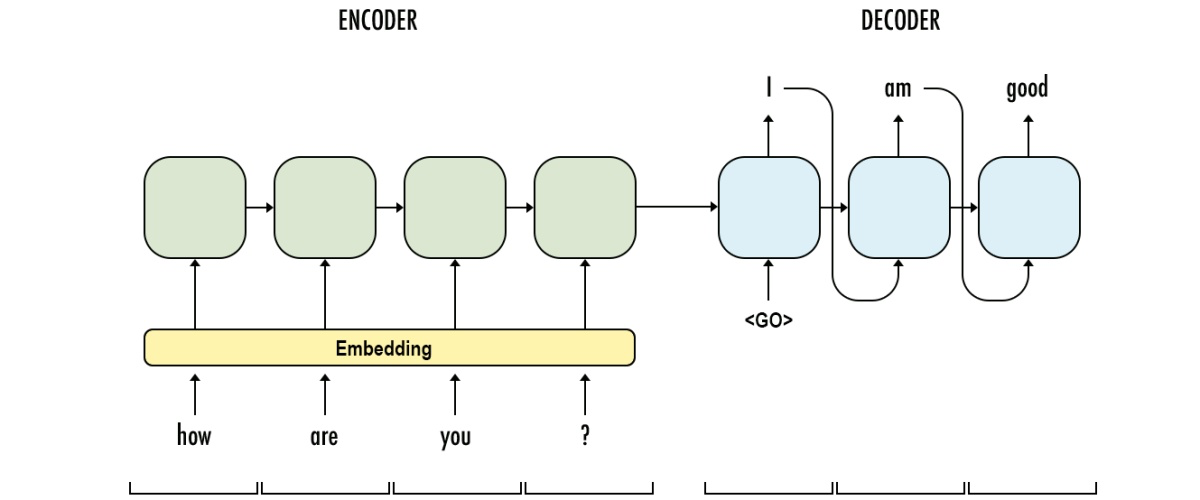
\includegraphics[width=1\textwidth]{seq2seq_model} %中括号中的参数是设置图片充满文档的大小,你也可以使用小数来缩小图片的尺寸。
    \caption{序列到序列模型} %caption是用来给图片加上图题的
    \label{seq2seq_model} %这是添加标签,方便在文章中引用图片。
\end{figure}%figure环境

而对于这类任务,序列到序列(Sequence to Sequence, Seq2Seq)模型被\cite{bahdanau2015neural}和\cite{sutskever2014sequence}先后提出。
序列到序列模型的经典结构如图\ref{seq2seq_model}所示,也被称为编码解码模型。
模型的编码器部分接收一段输入文本序列,然后将文本中的潜在信息编码到隐状态$h_i$中,最后输出最终的隐状态$h_t$作为文本的内容向量$c$,解码器则在文本向量$c$的帮助下预测对应的输出序列。
序列到序列模型克服了传统神经网络模型输入语句长度和输出语句长度。\cite{shang2015neural}使用序列到序列模型来完成短文本对话任务。

但是序列到序列模型面临四个困难:
模型不能参考历史对话来进行生成回复。
模型容易生成大量无意义、通用的语句作为回复。
模型没有结合世界知识,很难理解深层次语义。
对话系统应该根据对象的不同而采用不同的说话方式。

本文将在后续小结讨论解决这些困难的现有方法。

\subsubsection{利用历史信息}
编码具有上下文的信息,例如对话历史,能有效帮助模型生成前后一致、有信息量而且符合具体语境的回答,因为这些信息有助于模型更好地理解问题的语义和语境。但传统Seq2Seq模型面临无法对由多个句子构成的对话历史建模的现实困难,由此产生了一系列引入对话历史的模型。

\cite{sordoni2015a}通过将历史信息和用户查询通过全连接层进行编码,将其作为辅助的历史信息来指导解码器生成回答。
\cite{serban2016building}提出层次化序列到序列模型,在编码阶段对历史信息进行先后进行词级别编码和句子级编码,从而使得编码器能够在句子层面提取历史信息。
\cite{tian2017how}比较各种融合对话历史方法的优劣,并指出通过引入对话历史,有利于产生更长、更富信息和更多样化的回复,提高回复质量。
\cite{xing2018hierarchical}使用注意力机制来增强层次化模型对历史信息的提取能力,减少无关噪音。
\cite{serban2017a}在层次化模型中加入变分自编码器和记忆网络来跟踪对话的长期记忆。

\subsubsection{减少无意义语句}
生成式模型始终存在的挑战是其倾向于生成无意义的、缺少信息量的、通用回答\cite{li2016a}。
例如,对于任何的用户语句,生成的结果都有可能是“我也觉得”或“我也是这么认为的”这样、可以应用到几乎所有语句的“万能回答”。
无论模型在中文数据还是在英文数据上进行训练,这种现象都非常明显。

\cite{li2016a}提出互信息指标来作为生成句子的评价指标,从而在生成的候选回答中挑选出有意义的回答。
\cite{li2016deep, li2017adversarial}还通过引入强化学习,将MMI作为惩罚项来对生成器生成的无意义或重复语句进行惩罚。
\cite{shao2017generating}引入随机集束搜索来提高模型性能。
\cite{tian2017how}指出通过引入对话历史,有利于产生更长、更富信息和更多样化的回复
\cite{liu2018toward}通过使用基于统计的句子出现频率作为权重,来惩罚通用回答。
\cite{song2018an}提出结合检索模型挑选出的候选回答的方法,利用复制机制和多层次的attention机制来指导回复的生成。

\subsubsection{知识图谱}
在人们的对话交流中,往往会隐含对真实世界的假设。
对话系统也需要利用外部知识来增强模型对对话内容的理解和表示能力。
而且引入外部知识还能减少无意义语句的生成。

\cite{mou2016sequence}通过词对互信息指标挑选出关键词,然后将关键词用于指导回复的生成方向。
\cite{xing2017topic}利用LDA模型学习对话的主题表示,再结合注意力机制指导回复生成。
\cite{young2018augmenting}通过编码外部知识库的实体三元组来辅助对话中涉及实体属性的生成。
\cite{liu2018knowledge}提出知识扩散机制,同时利用知识库中的匹配实体和相似实体。
\cite{zhou2018commonsense}使用图注意机制来编码实体向量来指导语义提取和词语生成工作。
\cite{dinan2019wizard}使用记忆网络和Transformer来建模查询、对话历史和实体的交互关系。

\subsubsection{个性化系统}
如何让对话系统表现得和人一样是一项极具挑战性的任务。一方面,人与人之间的语言习惯各有千秋;另一方面,在现实人们的日常交流中,根据对方的身份和偏好来调整谈话的风格和策略是非常自然的行为。
面向人类性格的传统研究是基于BigFive模型\cite{goldberg1993the},所以早期建立个性化对话系统的工作\cite{mairesse2007personage}同样是基于BigFive模型。
但是依据BigFive来对个性进行描述是非常困难和需要昂贵代价的任务\cite{zheng2019personalized}。

在大数据驱动的文本生成视角下,替代的方法是通过显式或隐式的用户信息输入来辅助回复的生成,从而是回复具有个性化。
而且相较于对话系统自身的固有语言风格,如何让生成式对话系统根据对话对象的特点和习惯,理解对象的个性化需求,从而生成高效、贴切的语句,成为研究人员更为关注的问题\cite{luo2019learning}。

\cite{li2016a}通过将用户的向量化表示拼接到输入向量中,使得生成语句符合用户特点。
\cite{kottur2017exploring}延续Li的思路将模型应用到多轮对话任务上。
\cite{zheng2019personalized}通过简易的门机制将解码器输出$y_i$和用户特征向量结合,得到回复的第$i$个单词。
\cite{luo2019learning}引入用户的属性和相似用户的对话信息,并使用注意力机制将用户属性的独热表示向量用以指导对对话历史和相似用户对话信息的隐变量表示。

但该任务的难点还存在于现有的大多数数据集都不适用于个性化对话生成任务,\cite{zheng2019personalized, joshi2017personalization, zhang2018personalizing}开源针对个性化任务的对话数据集,解决了传统对话数据集缺少对话者信息标注的问题。
\cite{zhang2019neural}通过迁移学习来让对话系统在不同小规模数据集上学习到不同的语言风格。

\section{工业界对话系统}
\begin{figure}[h] %figure环境,h默认参数是可以浮动,不是固定在当前位置。如果要不浮动,你就可以使用大写float宏包的H参数,固定图片在当前位置,禁止浮动。
    \centering %使图片居中显示
    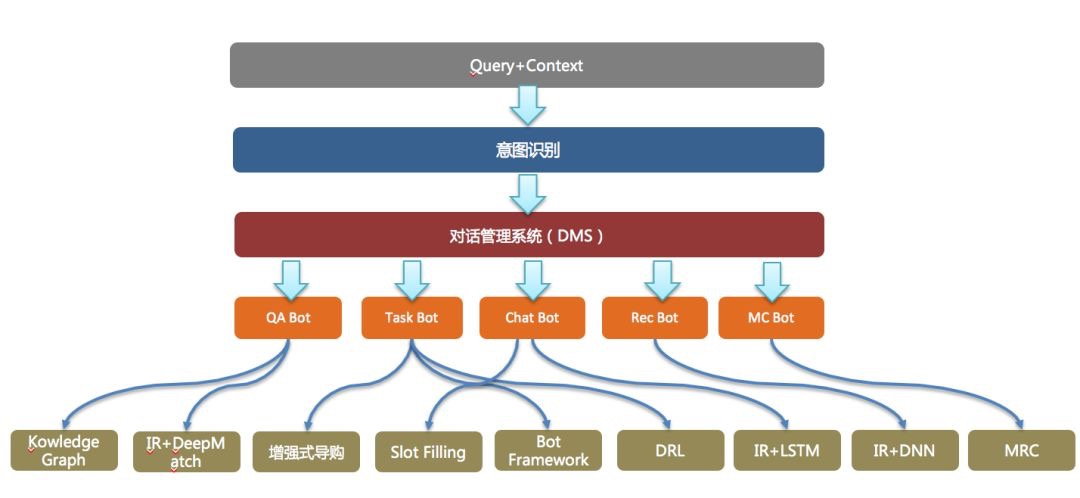
\includegraphics[width=1\textwidth]{industry_model} %中括号中的参数是设置图片充满文档的大小,你也可以使用小数来缩小图片的尺寸。
    \caption{阿里小蜜对话系统架构图} %caption是用来给图片加上图题的
    \label{industry_model} %这是添加标签,方便在文章中引用图片。
\end{figure}%figure环境

面对不同用户的多样化需求,工业界对话系统采用了多层次的管道结构\cite{li2019alime, zhou2018design},如图\ref{industry_model}所示。
通过预先的意图识别模块,将用户导向不同功能的对话系统,从而完成不同难度的语义理解和意图完成工作。
对于意图是“闲聊”的用户,通过闲聊型对话系统来基于语料库检索或生成回复\cite{zhou2018design}。
对于意图是“查询”的用户,通过与外部数据库和知识图谱相连接的问答型对话系统,使用文本匹配方法来检索相应回复模版\cite{li2019alime}。
对于意图是“请求”的用户,通过任务型对话系统基于会话状态来生成回复。

具体的对话系统结构和前文一致。

\section{总结} % 修改此处
构建能像人一样与人自然流畅交流的对话系统是人工智能领域的最高目标之一。
在人们的日常生活中,对话系统也能发挥出重要作用,如虚拟助手、智能客服等。
随着海量数据的产生和深度学习的发展,对话系统迎来了长足的发展。
本文沿着对话系统的历史发展脉络,介绍多种对话系统的构建方式,并评价了其优缺点。
本文简单介绍了工业界对话系统的架构,尝试为研究人员建立较为完整的研究视角。

% \starttwocolumn
\bibliography{citation} % 修改"mypaper.bib"文件

\end{document}
